\chapter{Electric Dipole Moment of Leptons}
\label{ch:leptonEDM}

Following the framework laid out previously, we want to perform EDM calculations on the various leptons.
However, we shall ignore the neutrinos. 
Thoretically, they are neutral and massless, thus they \emph{at best} will receive EDM contributions from the charged-Higgs related processes,
and are of lower theoretical significance.
Experimentally, EDM experiments are low-energy in nature, and low-energy manipulation of neutrinos is currently experimentally unfeasable.
We will thus focus our calculations on the electron and its cousins, the muon and the tau.
Any subsequent mention of ``leptons'' in this work will also by default only be referring to these three leptons. 
In the following sections of this chapter, we will first give a brief overview of the current experimental status,
then present our theoretical predictions of the EDMs of the electron, muon, and tau respectively.

\section{Experimental Overview}
A brief overview of current experimental bounds and projected future experimental sensitivity is given in \tabref{tab:leptonEDMExperiments}.
\begin{table}[thp]
    \centering
    \begin{adjustbox}{center}
        \begin{small}
            \begin{tabular}{cclcl}
                \toprule
                Lepton & \multicolumn{2}{c}{Current bound (\(e \) cm)} & \multicolumn{2}{c}{Future sensitivity (\(e \) cm)}\\
                \midrule
                Electron & \num{4.1e-30} & JILA~(2023)~\cite{JILA2023eEDM} & & \\
                & \num{1.1e-29} & ACME~(2018)~\cite{ACME2018eEDM} & & \\
                Muon & \num{1.8e-19} & BNL~(2009)~\cite{BNL2009MuonEDM} & \(\sim \num{e-21} \) & FNAL~\cite{Fermilab2016MuonEDM}, J-PARC~\cite{JPARC2019MuonEDM} \\
                & \(\sim \num{2e-20} \) & Pospelov~(2022)~\cite{Pospelov2022MuonEDM} & \(\sim \num{6e-23} \) & PSI~\cite{PSI2021MuonEDM} \\
                Tau & \(\Re\,d_{\tau} = \) \num{-0.62(0.63)e-17} & Belle (2003)~\cite{Belle2003TauEDM} & \(\sim \num{e-18}-\num{e-19} \) & Belle II~\cite{BelleII2019Projections} \\
                & & & \(\sim \num{0.7e-19} \) & Bernreuther~\cite{Bernreuther2021TauEDM}\\
                & \(\Im\,d_{\tau} = \) \num{-0.40(0.32)e-17} & Belle (2003)~\cite{Belle2003TauEDM} & \(\sim \num{e-18}-\num{e-19} \) & Belle II~\cite{BelleII2019Projections} \\
                & & & \(\sim \num{0.4e-19} \) & Bernreuther~\cite{Bernreuther2021TauEDM} \\
                \bottomrule
            \end{tabular}
        \end{small}
    \end{adjustbox}
\caption{Overview of current bounds and future sensitivities for lepton EDMs.}
\label{tab:leptonEDMExperiments}
\end{table}

As can be seen in the table, the experimental development of electron EDM ({\eedm}) over the past few years has been remarkably rapid.
Just earlier in 2023, JILA~\cite{JILA2023eEDM} has surpassed the previous bound from ACME~\cite{ACME2018eEDM} and pushed the precision of {\eedm} down to \(|d_{e}| < \num{4.1e-30} \ecm\) .
It is noteworthy to point out that these {\eedm} experiments are relatively small in scale, ``tabletop experiments'' even when compared to behemoths like the LHC, which makes the extreme precision achieved all the more impressive.
The smallness of {\eedm}, courtesy of this precision, has put significant pressure on the theoretical side of baryogenesis CPV parameter spaces.
In~\secref{sec:eEDM} we shall establish in {\gthdm} a way to maintain adequate baryogenesis efficiency while evading the experimental {\eedm} bounds.

For the muon, the leading experimental bound on muon EDM ({\muedm}) is by the Muon g-2 experiment at Brookhaven National Laboratory (BNL)~\cite{BNL2009MuonEDM}, giving us the bound
\(|d_{\mu}| < \num{1.8e-19} \ecm\).
There is also an indirect limit derived from the ACME 2018 {\eedm} bound, which is claimed~\cite{Pospelov2022MuonEDM} to be \(\sim \num{2e-20} \ecm\).
There are several experiments that aim to search for {\muedm} in the forseeable future.
The Fermilab (FNAL) Muon g-2~\cite{Fermilab2016MuonEDM} and J-PARC Muon g-2/EDM~\cite{JPARC2019MuonEDM} experiments project their sensitivities at \(\sim \num{e-21} \ecm\),
while another experiment at PSI~\cite{PSI2021MuonEDM} aims to improve by an additional order of magnitude,
reaching \(\sim \num{6e-23} \ecm\).
With these experiments on the horizon, the prospects for {\muedm} in the coming decade do look rather promising.

As for the tau, tau EDM ({\tauedm}) measurements are far less precise given the short lifetime of the tau lepton.
The most prominent method to derive the limits are from spin-momentum correlations of final state decay products in the \(e^{+}e^{-} \to \gamma^{*} \to \tau^{+}\tau_{-}\) process,
where {\tauedm} enters the matrix element of the \(\tau\tau\gamma \) vertex.
The current best limit is by Belle~\cite{Belle2003TauEDM}, with the real and imaginary parts given seperately, both at \(\sim \num{e-17} \).
Just as with {\muedm}, an indirect limit can be derived from {\eedm} as per~\cite{Pospelov2022MuonEDM} (not listed here).
Belle II~\cite{BelleII2019Projections} projects an order-of-magnitude improvement to the Belle bounds.
On the other hand, some improvement is possible by studying ``optimal'' observables, as per~\cite{Bernreuther2021TauEDM}.

If we assume that new physics (NP) contributions scale with \(m_{l} \) (such as models~\cite{DAmbrosioEtAl2002MFV} with minimal flavor violation (MFV)),
we can make back-of-the-envelope estimates of the ``equivalent precision'' bounds for {\muedm} and {\tauedm} from the current {\eedm} bound.
Applying the scaling \(|d_{\mu(\tau)}/d_{e}| \simeq m_{\mu(\tau)}/m_{e}\) to the JILA bound in~\tabref{tab:leptonEDMExperiments}, 
we can obtain the equivalent precision bounds \(|d_{\mu}| \sim \num{8.5e-28} \ecm\) and \(|d_{\tau}| \sim \num{1.4e-26} \ecm\), respectively.
Referring back to \tabref{tab:leptonEDMExperiments}, the projected sensitivities for {\muedm} fall just shy of 5 orders of magnitude short,
while those for {\tauedm} are still st least 7 orders of magnitude away.
However, if the flavor dynamics are quite different, this \(m_{l} \) scaling might not hold~\cite{HillerEtAl2010MuonEDMfromFlavor, CrivellinEtAl2018MuonEDMg-2},
possibly leading to larger \(d_{\mu} \) and \(d_{\tau} \). 
In~\secref{sec:muEDM}~and~\secref{sec:tauEDM} we shall see how {\gthdm} gives rise to larger \(d_{\mu} \) and \(d_{\tau} \), respectively,
while still maintaining the possibility of yielding a smaller value should the bounds close in.

\section{The Electron}\label{sec:eEDM}
For the electron, an extensive study of {\eedm} in {\gthdm} can be found in the 2018~\cite{FHS2018EWBGandEDM} and 2020~\cite{FHS2020EDMCancellation} papers of Fuyuto, Hou, and Senaha.
Our investigation on {\eedm}~\cite{HKT2024eEDMnEDM} is essentially an extension of the 2020 paper to a larger parameter space.

\subsection{Cancellation Mechanism}\label{sec:eEDM-cancellation}
As mentioned in \secref{sec:EWBG}, one big motivation for {\gthdm} as a viable model is the fact that \(\order{1} \rho_{tt}\) can drive baryogenesis through \(\lambda_{t}\Im\rho_{tt} \).
However, this same \(\rho_{tt} \), along with \(\rho_{ff} \) for a given fermion \(f \), also generates EDM for said fermion (\secref{sec:g2hdm_in_edm}).
We thus arive at a ``point of tension'' between theory and experiment:
we desire a large \(\rho_{tt} \) for baryogenesis, but need a small \(\rho_{tt} \) to survive precision bounds on various EDMs.
Electron EDM, in particular, is a great ``observable of contention'', since experiments measuring it are the most precise compared to other EDMs.
In an attempt to address this issue, Fuyuto, Hou, and Senaha proposed a ``cancellation ansatz'' between \(\rho_{ee} \) and \(\rho_{tt} \) 
\begin{equation}\label{eq:ansatz}
    \Re\rho_{ee} = -r\frac{\lambda_{e}}{\lambda_{t}}\Re\rho_{tt} \text{, } \quad \Im\rho_{ee} = +r\frac{\lambda_{e}}{\lambda_{t}}\Im\rho_{tt},
  \end{equation}
which facilitates a ``cancellation mechanism'' that allows for small values of {\eedm} while keeping a \textit{sizeable} \(\rho_{tt} \).
The ``cancellation'' in this mechanism arises from the opposite signs of the \(W \)-loop and the top-loop in the Barr-Zee diagrams.
Referring to~\eqnref{eq:BarrZee-phiG-toploop}~and~\eqnref{eq:BarrZee-cHW-Wloop}, we can see that
\begin{align}
    (d^{\phi G}_{l})_{t} = -&\frac{e\,m_{l}}{(4\pi)^{4}}\sqrt{2}G_{F}\sum_{\phi=h,H,A}\sum_{G=\gamma,Z}(\rho \text{ couplings})(\text{Loop functions}) \\
    (d^{\phi G}_{l})_{W} = +&\frac{e\,m_{l}}{(4\pi)^{4}}\sqrt{2}G_{F}\sum_{\phi=h,H,A}\sum_{G=\gamma,Z}(\rho \text{ couplings})(\text{Loop functions})
\end{align}
thus the effectiveness of such a cancellation is determined by the relationship between the new \(\rho \) couplings and the loop functions of the Barr-Zee diagrams.
In the case of total cancellation, \((d^{\phi G}_{l})_{t} = -(d^{\phi G}_{l})_{W}\), we obtain
\begin{equation}\label{eq:exact-cancellation}
    \frac{\Im\rho_{ee}}{\Im\rho_{tt}} = c \times \frac{\lambda_{e}}{\lambda_{t}} \text{, } \quad \frac{\Re\rho_{ee}}{\Re\rho_{tt}} = \frac{\Im\rho_{ee}}{\Im\rho_{tt}},
\end{equation}
where \(c = (16/3)\Delta g /(\Delta \mathcal{I}_{W}^{\gamma}-(16/3)\Delta f + \epsilon) \), 
\(\Delta X = X(m_{t}^{2}/m_{h}^{2}) - X(m_{t}^{2}/m_{H}^{2}) \), 
and \(s_{2\gamma}\lambda_{t}\epsilon = -(16/3)\Re{\rho_{tt}}[f(m_{t}^{2}/m_{A}^{2})+g(m_{t}^{2}/m_{A}^{2})] \).
This value of \(c \) is thus only dependent on the loop functions and the heavy Higgs masses.
For \(m_{h} = \SI{125}{\GeV} \) and \(m_{H} = m_{A} = \SI{500}{\GeV } \), \(c \simeq 0.71 \)
Rearranging~\eqnref{eq:exact-cancellation},
and changing the exact cancellation value \(c \) to a variable prportionality parameter \(r \),
gives us the form of the cancellation ansatz.
This ansatz signifies two key points.
First, it gives a flavor hierarchy \(|\rho_{ee}|/|\rho_{tt}|\sim\lambda_{e}/\lambda_{t} \) that reflects SM.
Second, it represents a phase lock between \(\rho_{ee} \) and \(\rho_{tt} \).
With our working assumption of Higgs masses, this ansatz results in a ``dip'' in {\eedm} around the \(r \) value of \(\sim 0.7 \),
which is when complete cancellation occurs between the \(W \)-loop and the top-loop.
This provides a mechanism for the {\eedm} in {\gthdm} to be small and evade the experimental bounds while not directly modifying \(\rho_{tt} \).

\subsection{Enlarging the Parameter Space}
When revisiting their study, we found the assumptions on the value of \(\rho_{tt} \) to be quite ``conservative'', setting \(\Re\rho_{tt} = \Im\rho_{tt} = -0.1 \) (which equates to \(|\rho_{tt}| = 0.1\sqrt{2} \approx 0.14\)).
We believe that might be due to \textit{playing it safe} under the pressure of the rapid advancements on the experimental front. 
In our study~\cite{HKT2024eEDMnEDM}, we \textit{push against the boundary}, and explore a larger range of \(\rho_{tt} \), up to \(\Re\rho_{tt} = \Im\rho_{tt} = -0.3 \) (\(|\rho_{tt}| = 0.3\sqrt{2} \approx 0.42\)). 
We want to see how big we can keep the parameter space for baryogenesis while still satisfying precision constraints.
As mentioned before, one of the key points of {\gthdm} is the \textit{flavor hierarchy}, illustrated by the \textit{rule of thumb}~\eqnref{eq:ruleofthumb}.
This ``cancellation ansatz'' happens to capture the idea of such a hierarchy pretty well from a numerical standpoint; 
so, for the sake of numerical illustration of the flavor hierarchy, we extend the ansatz to all fermion \(\rho_{ff} \)s, except for the top itself:
\begin{equation}\label{eq:ansatz-extended}
    \Re\rho_{ff} = -r\frac{\lambda_{f}}{\lambda_{t}}\Re\rho_{tt} \text{, } \quad \Im\rho_{ff} = +r\frac{\lambda_{f}}{\lambda_{t}}\Im\rho_{tt}.
\end{equation}
We must reiterate that this is merely a move of convenience, and the actual values of the \(\rho_{ff} \)s need not precisely match this ansatz.
Results are shown in \figref{fig:eEDM}.
% Figure: eEDM cancellation results
For the sake of clarity, we have taken a slight liberty in illustrating the range of the purple ``allowed window'' band,
using the left- and right-most curves instead of the left and right side of a given curve.
Nevertheless, the trend we wish to describe is not affected by such.
From our results, it can be seen that as \(|\rho_{tt}| \) increases, the allowed window of the proportionality parameter \(r \) shrinks, yet there is still a decent range of acceptable probable values.
\(\Re\rho_{tt} = \Im\rho_{tt} = -0.1 \) was indeed a conservative representative value, and \(\Re\rho_{tt} = \Im\rho_{tt} = -0.3 \) may still be a viable option in the baryogenesis parameter space.

\section{The Muon}\label{sec:muEDM}
After the electron, we move on to its slightly heavier cousin, the muon. 
Since the bound on the muon is not as strong, one does not need to resort to the cancellation ansatz immediately.
Instead, we perform a scan of the \(\rho_{tt} \) parameter space for a representative \(\rho_{\mu\mu} \) value, and see how it affects the \(\mu \)EDM.
Results are shown in \figref{fig:muEDM}.
% Figure: muonEDM results
We see that there is still a ``cancellation dip'' for the neutral scalar-attached loops, which arises from the opposite signs of the \(W \)-loop and the top-loop.
The details of said cancellation is exactly the same as that of the electron.
Our predicted values for \(\mu \)EDM are still two to three orders of magnitude below the current bounds, so we are eager to see development on the experimental front.
Once the bounds close in, it may also be fruitful to consider the ``cancellation ansatz'' on the muon as well, especially since the leptons share a extra Yukawa matrix \(\rho^{l} \),
which makes it more likely that the \(\rho_{ll} \) might exhibit similar relationships with \(\rho_{tt} \).

\section{The Tau Lepton}\label{sec:tauEDM}
Lastly, we analyze the heaviest lepton, the tau.
On the experimental front, the precision of tau EDM (\(\tau \)EDM) measurements are still pretty low.
We perform the same calculations as the muon, with \(\rho_{\mu\mu} = i\lambda_{\mu} \) replaced by \(\rho_{\tau\tau} = i\lambda_{\tau} \).
Results are shown in \figref{fig:tauEDM}.
% Figure: tauEDM results
As seen in the figure, our predicted values are still several orders of magnitude below current experimental results.
Further precision or methodology improvements are required for a more fruitful analysis of \(\tau \)EDM, so we just present our results here without much further comment.

\clearpage
% eEDM cancellation results
\begin{figure}[p]
    \centering
    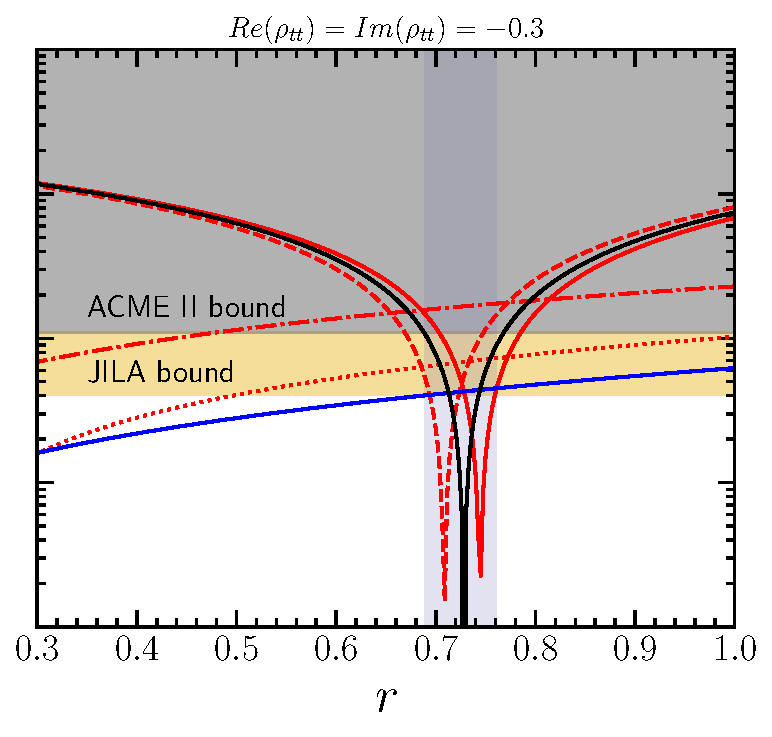
\includegraphics[width=6.95cm,height=5.55cm,angle=90]{fig2_3.pdf}\\
    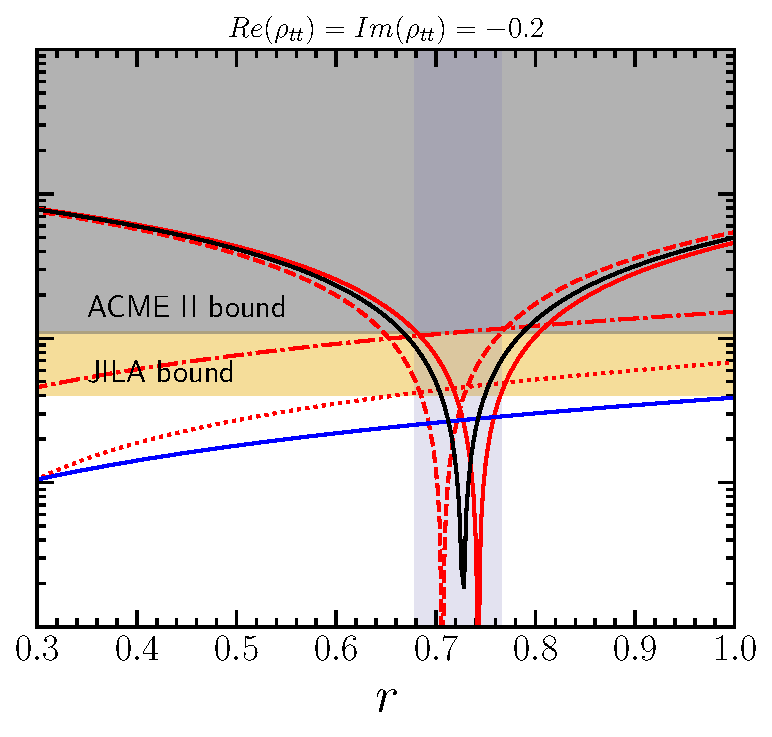
\includegraphics[width=6.95cm,height=5.55cm,angle=90]{fig2_2.pdf}\\
    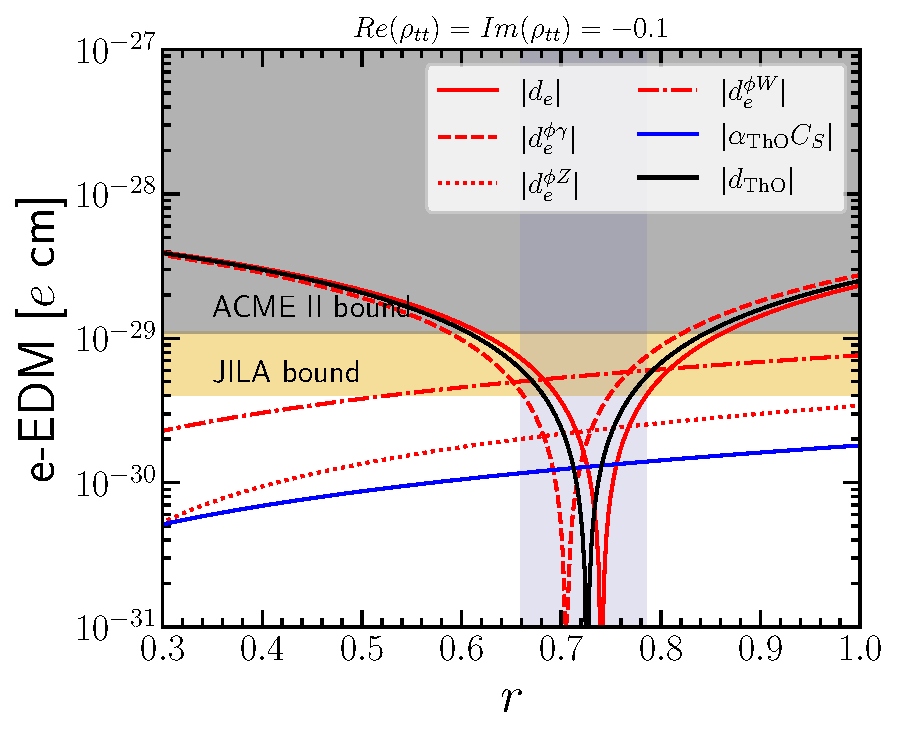
\includegraphics[width=7.95cm,height=5.55cm,angle=90]{fig2_1.pdf}
    \caption{eEDM v.s. \(r \) for a larger range of \(\rho_{tt} \) with ansatz~Eq.~\eqref{eq:ansatz-extended}. (\(c_{\gamma} = 0.1, m_{H, A, H^+} = 500\,\mathrm{GeV} \))}
    \label{fig:eEDM}
\end{figure}

% muonEDM results
\begin{figure}[p]
    \centering
    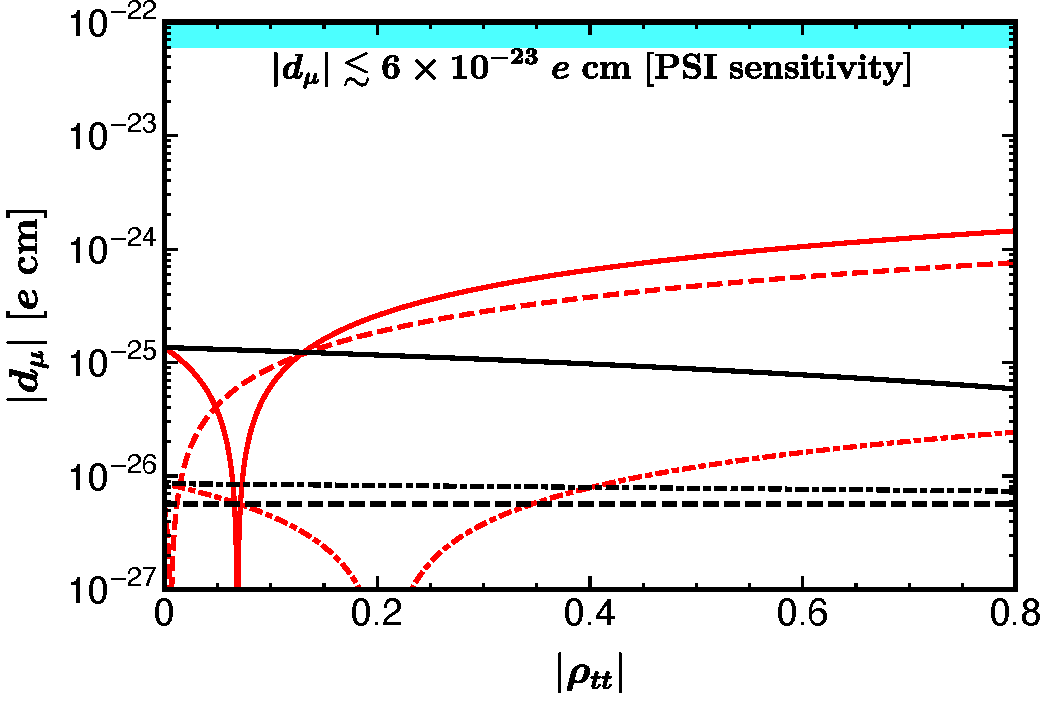
\includegraphics[width=0.7\textwidth]{muEDM.pdf}
    \caption{\(\mu \)EDM results.}
    \label{fig:muEDM}
\end{figure}

% tauEDM results
\begin{figure}[p]
    \centering
    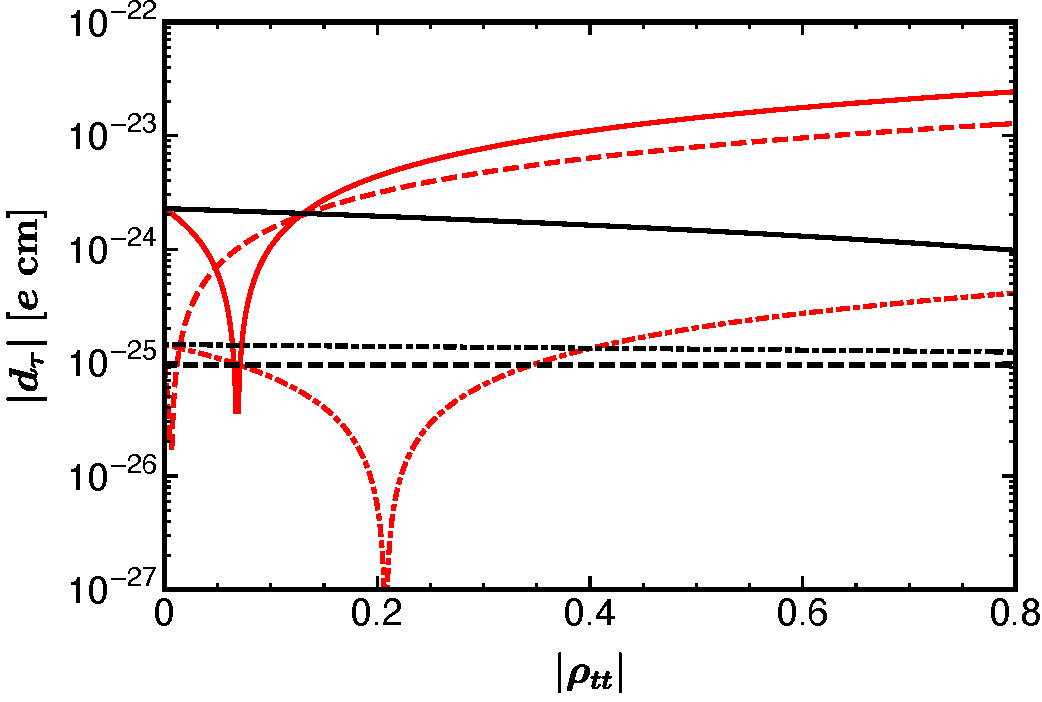
\includegraphics[width=0.7\textwidth]{tauEDM.pdf}
    \caption{\(\tau \)EDM results.}
    \label{fig:tauEDM}
\end{figure}